\subsection{Mixed runs}
Getting normalised data from~\cite{Betel2018} available as a dataset~\cite{Wang2017}. it is possible to analyse health and diseased at the same time.

It is 
\begin{figure}[htb!]
    \centering
    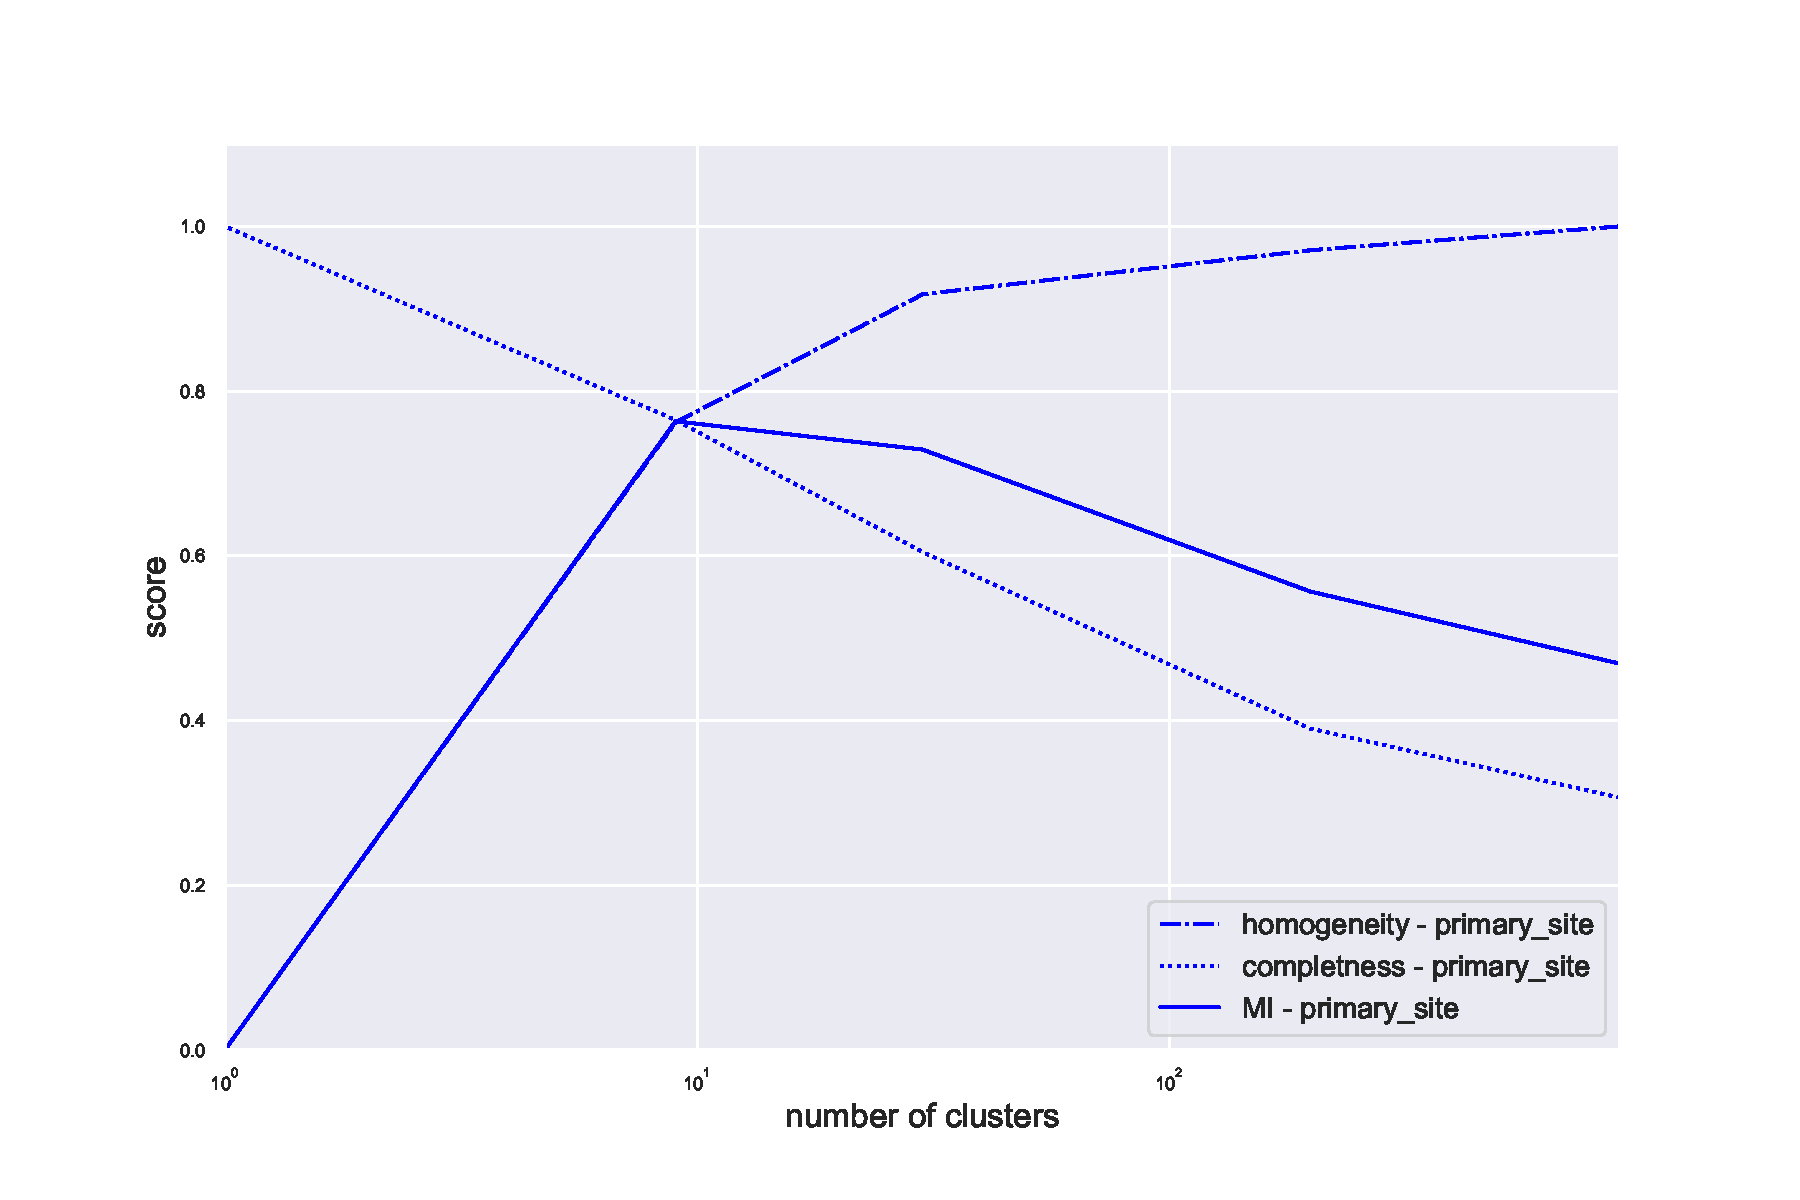
\includegraphics[width=0.8\linewidth]{pictures/topic/merged/metric_scores_primarysite.pdf}
    \caption{Caption}
    \label{fig:topic/merged/metric_scores_primarysite}
\end{figure}

\begin{figure}[htb!]
    \centering
    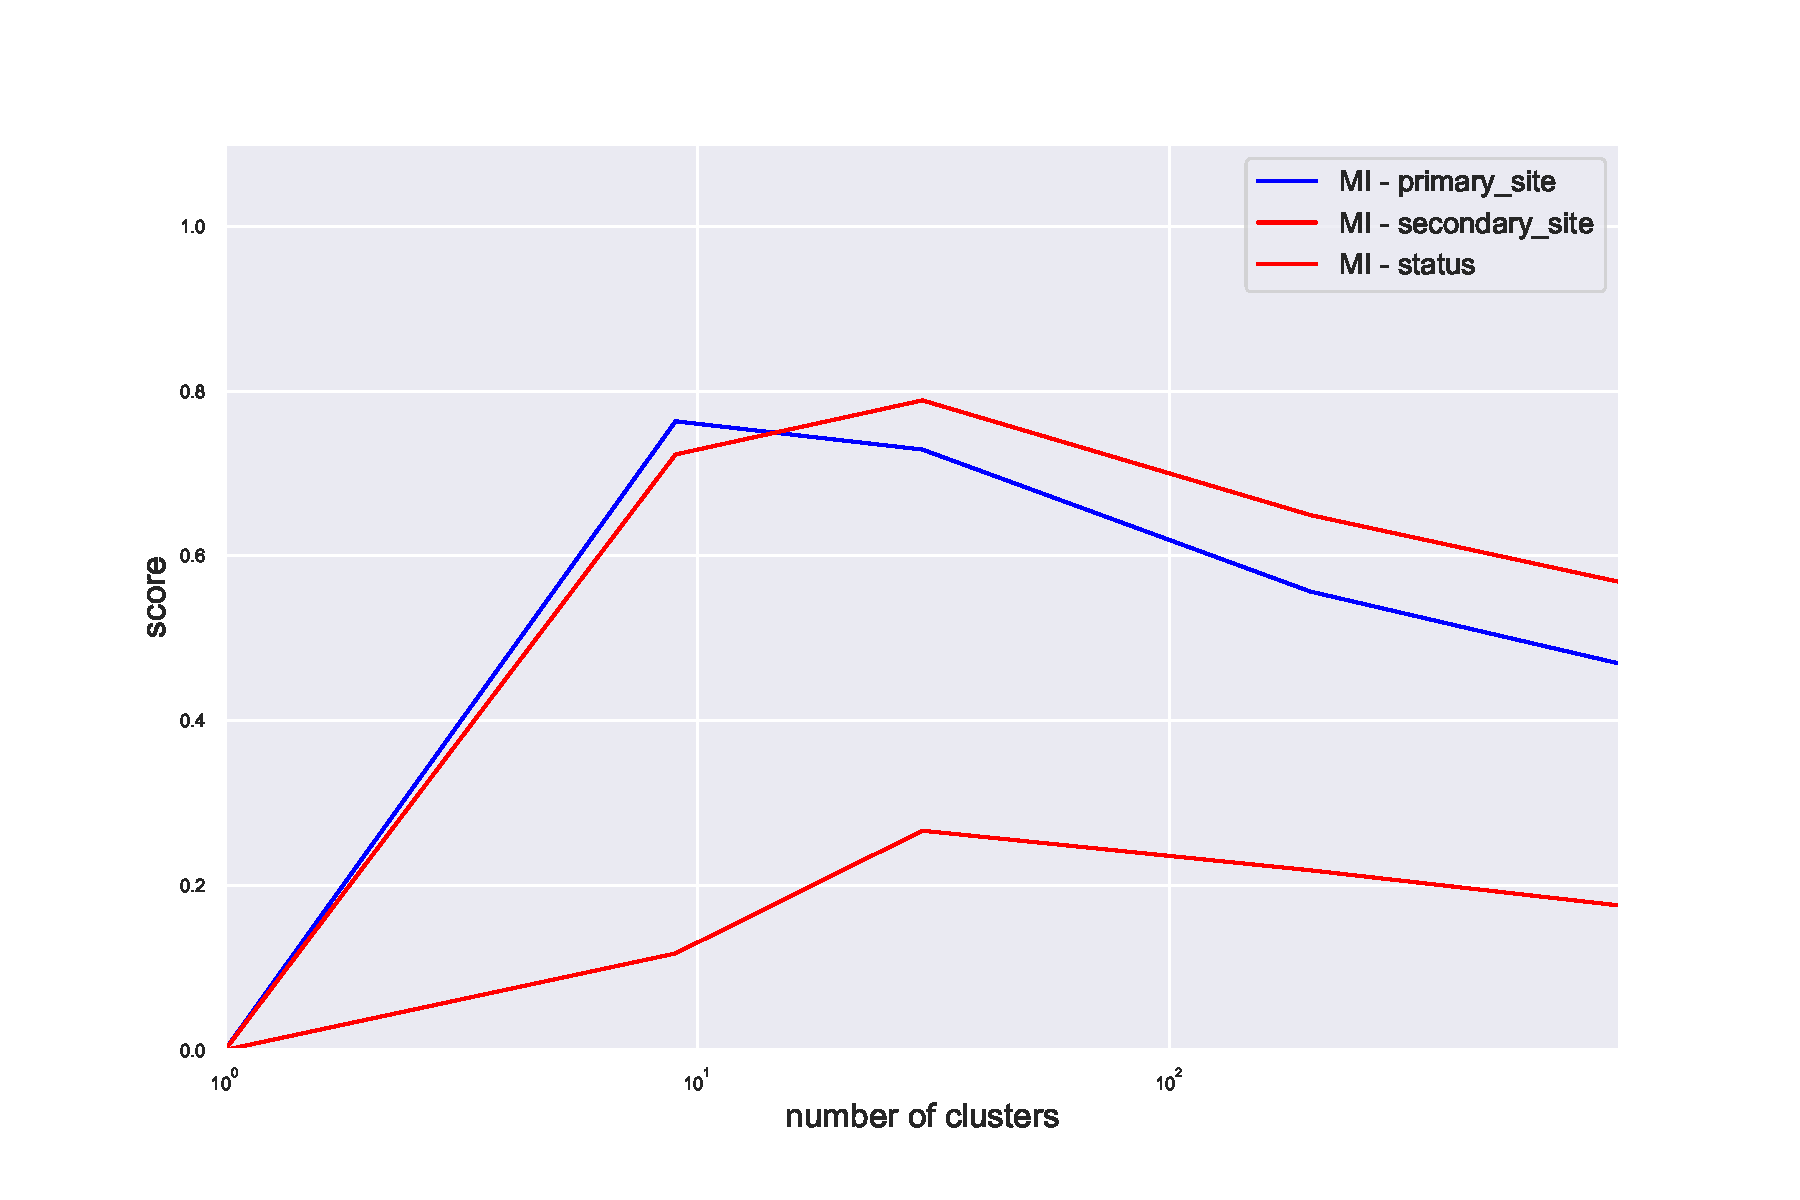
\includegraphics[width=0.8\linewidth]{pictures/topic/merged/metric_scores.pdf}
    \caption{Caption}
    \label{fig:topic/merged/metric_scores}
\end{figure}

\begin{figure}[htb!]
    \centering
    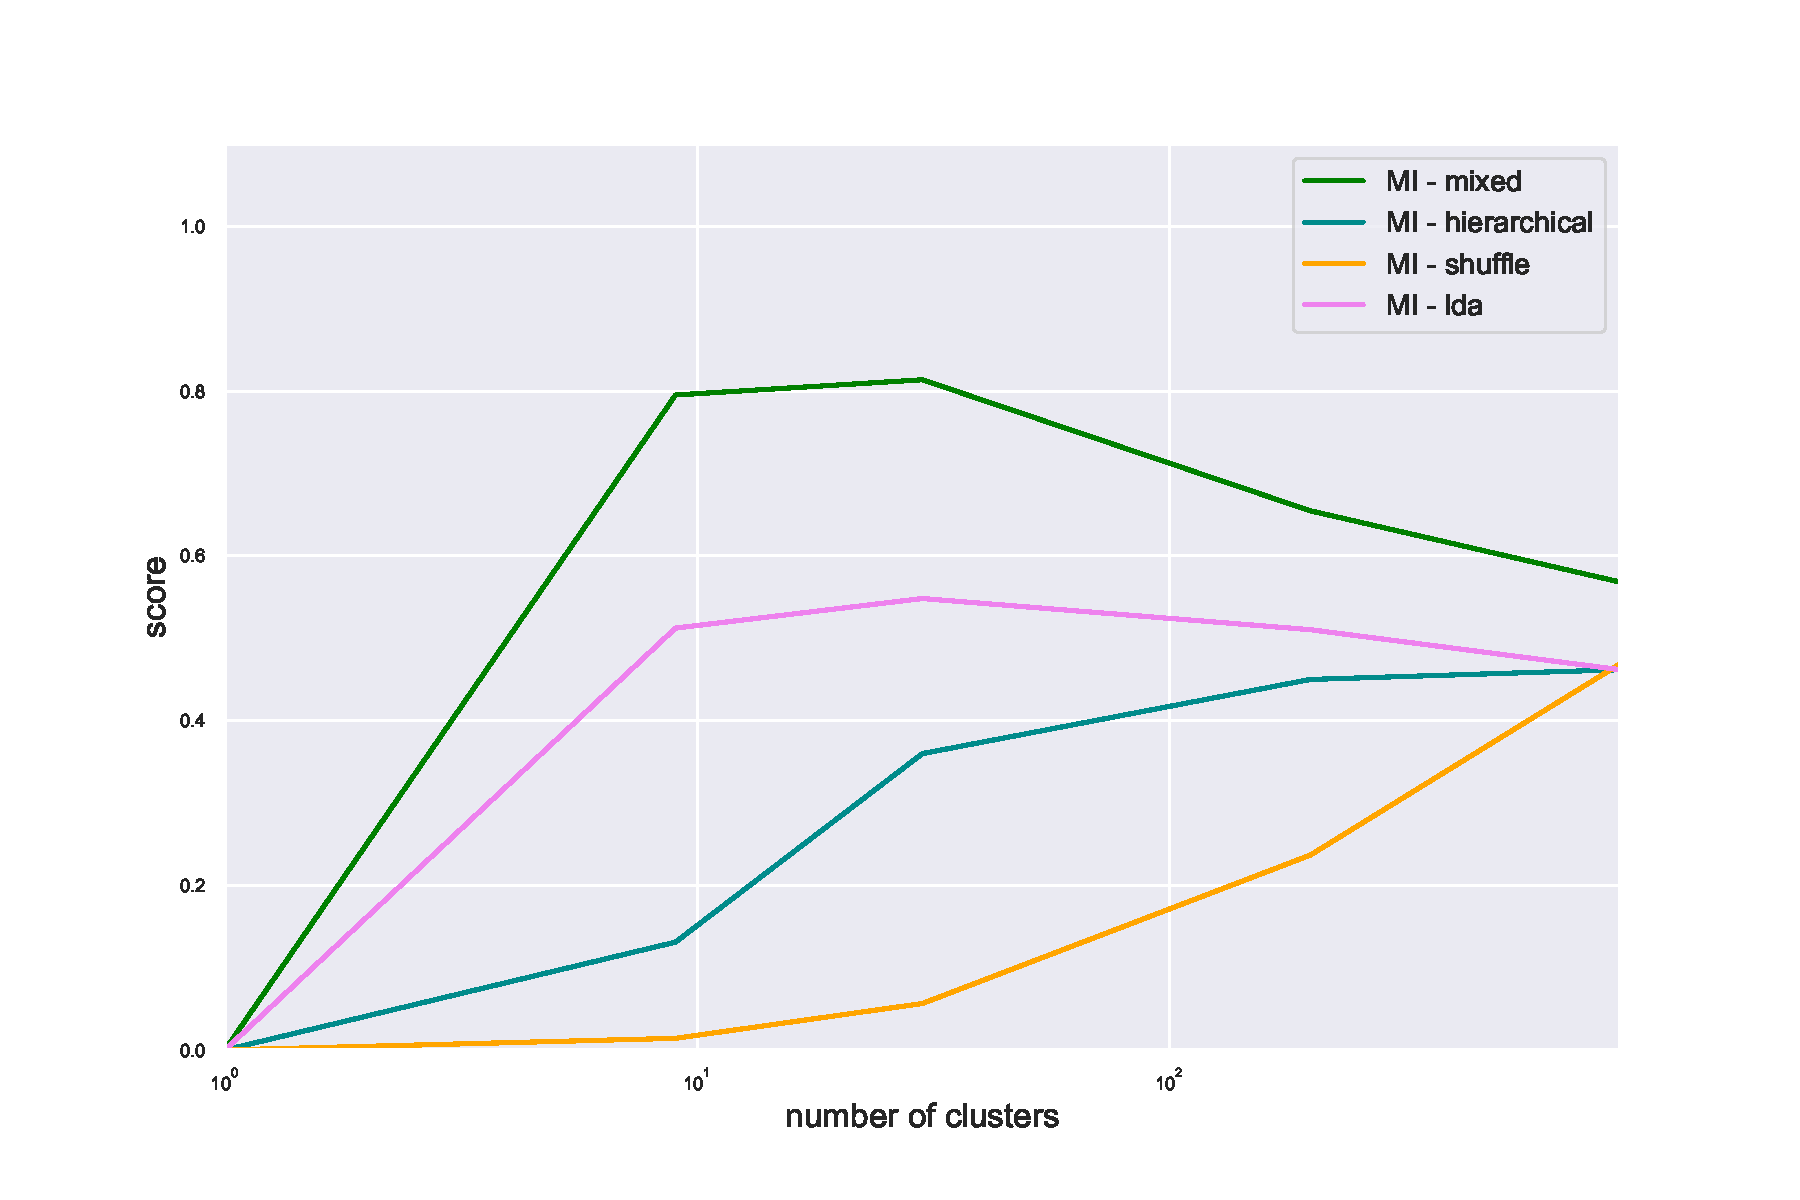
\includegraphics[width=0.8\linewidth]{pictures/topic/merged/metric_scores_all.pdf}
    \caption{Caption}
    \label{fig:topic/merged/metric_scores_all}
\end{figure}

\begin{figure}[htb!]
    \centering
    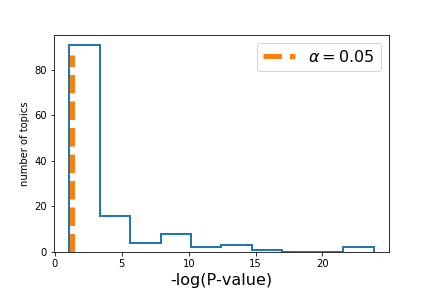
\includegraphics[width=0.8\linewidth]{pictures/topic/merged/pvaluescrosstopic.png}
    \caption{Caption}
    \label{fig:topic/merged/pvaluescrosstopic}
\end{figure}


\begin{figure}[htb!]
    \centering
    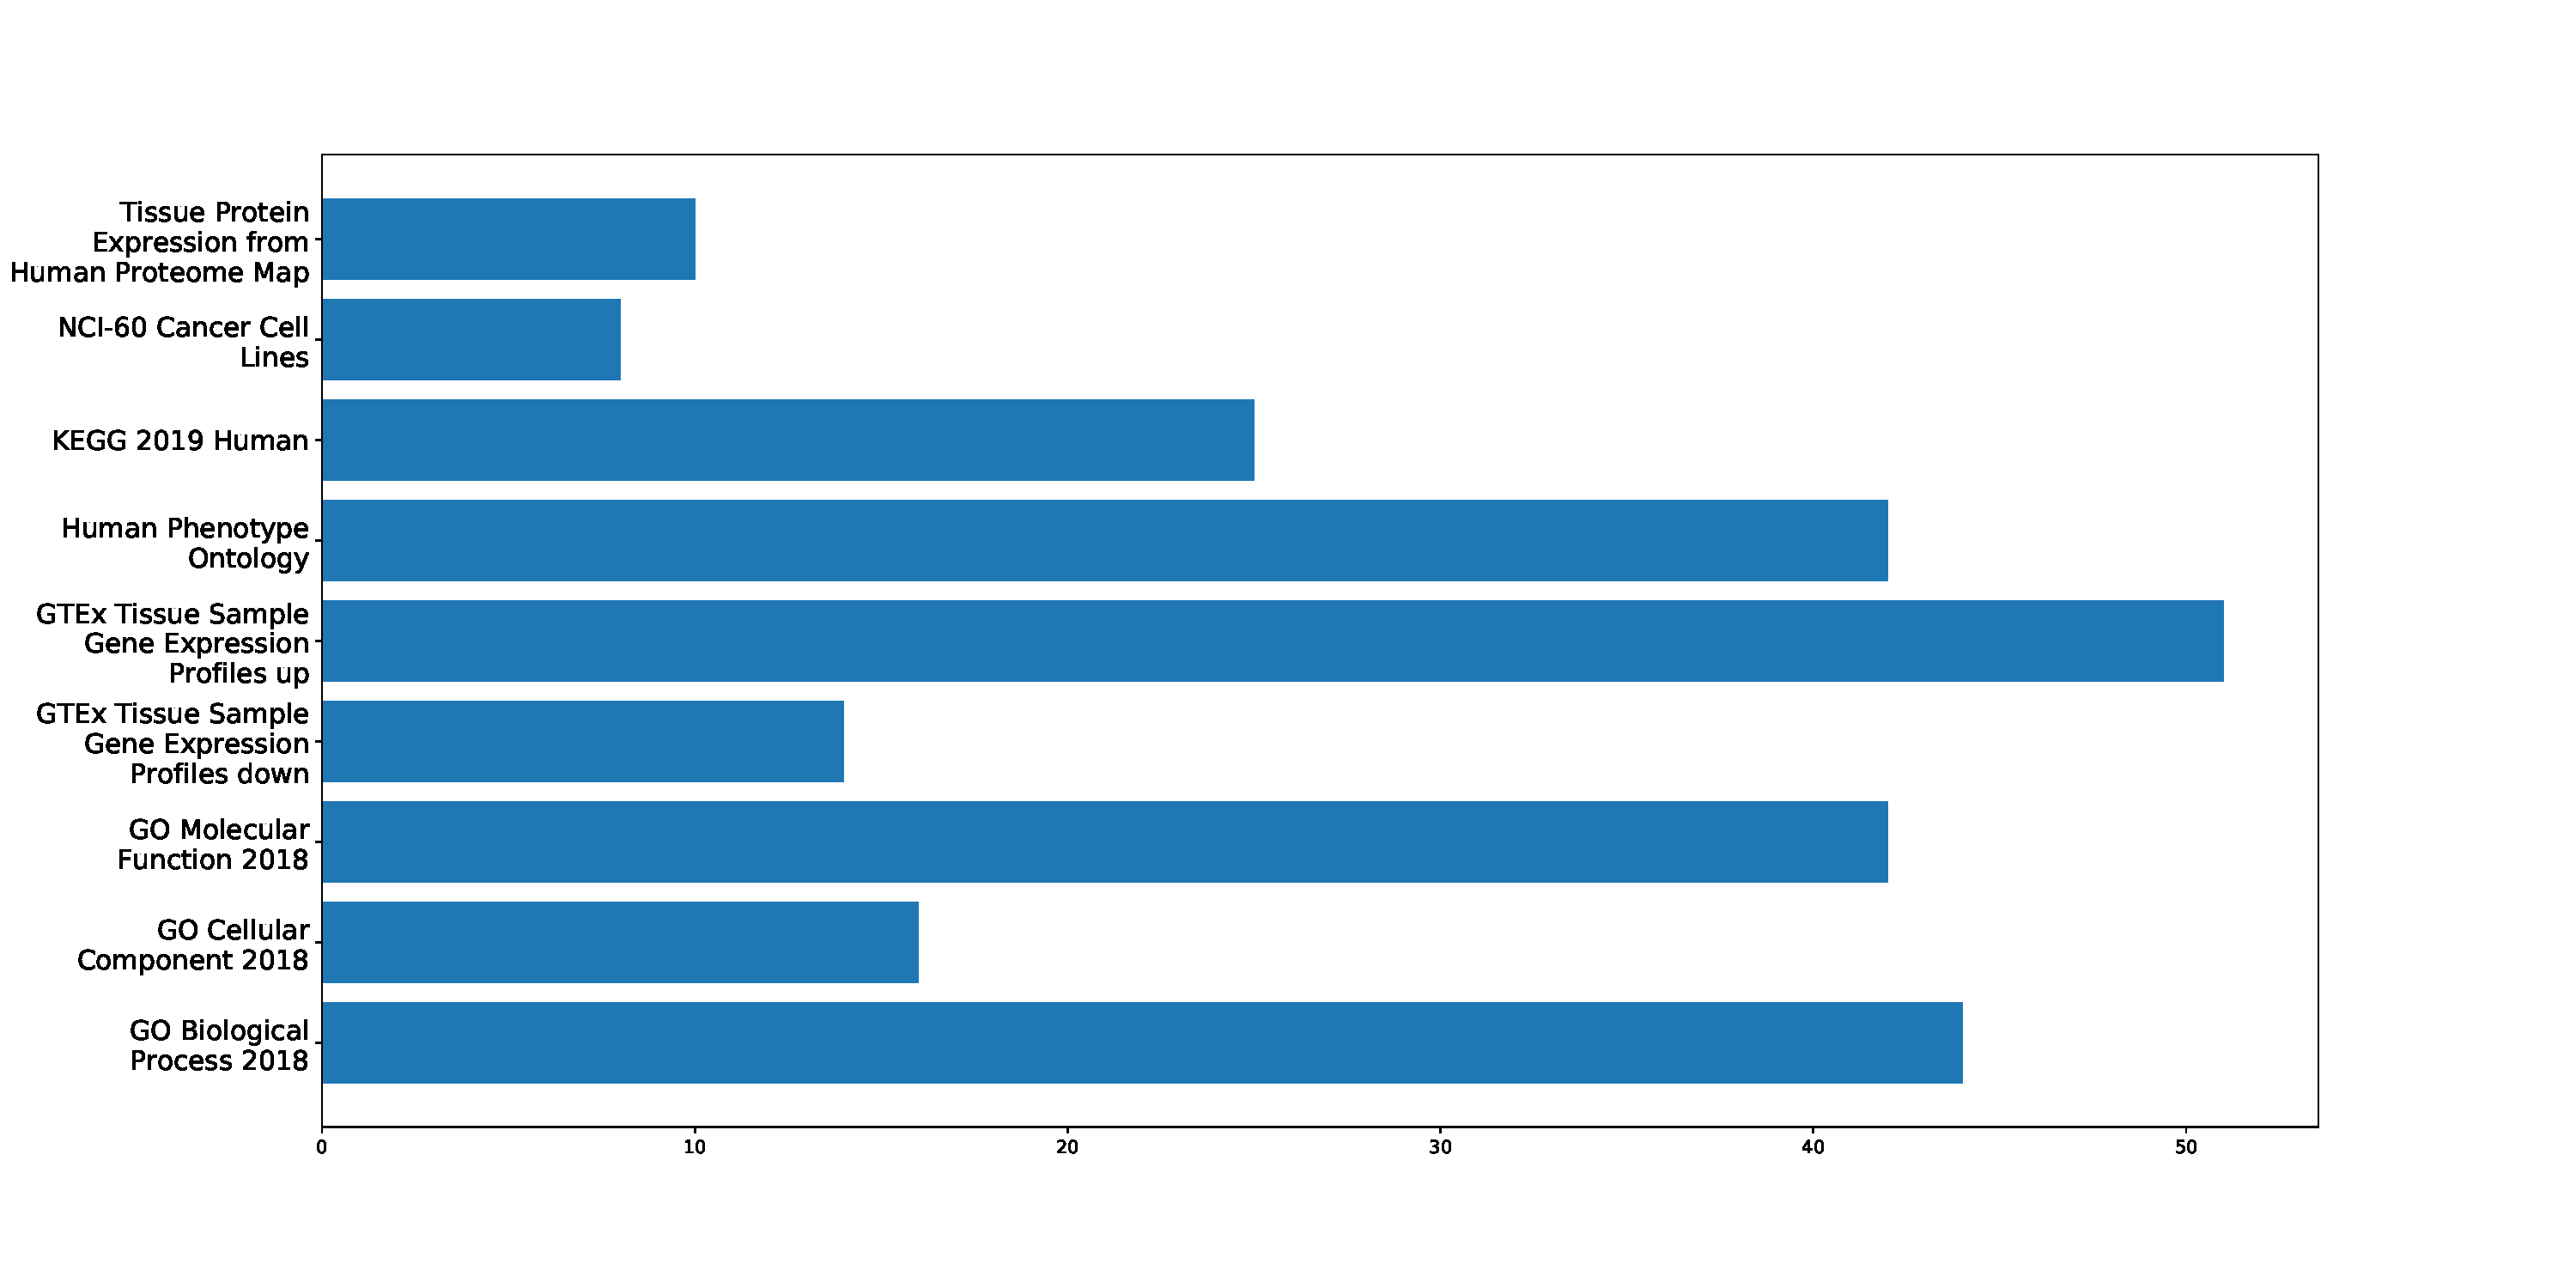
\includegraphics[width=0.8\linewidth]{pictures/topic/merged/pvaluecategories.pdf}
    \caption{Caption}
    \label{fig:topic/merged/pvaluecategories}
\end{figure}

DAVID~\cite{huang2008bioinformatics,huang2009systematic} confirms analogous result
\begin{figure}[htb!]
    \centering
    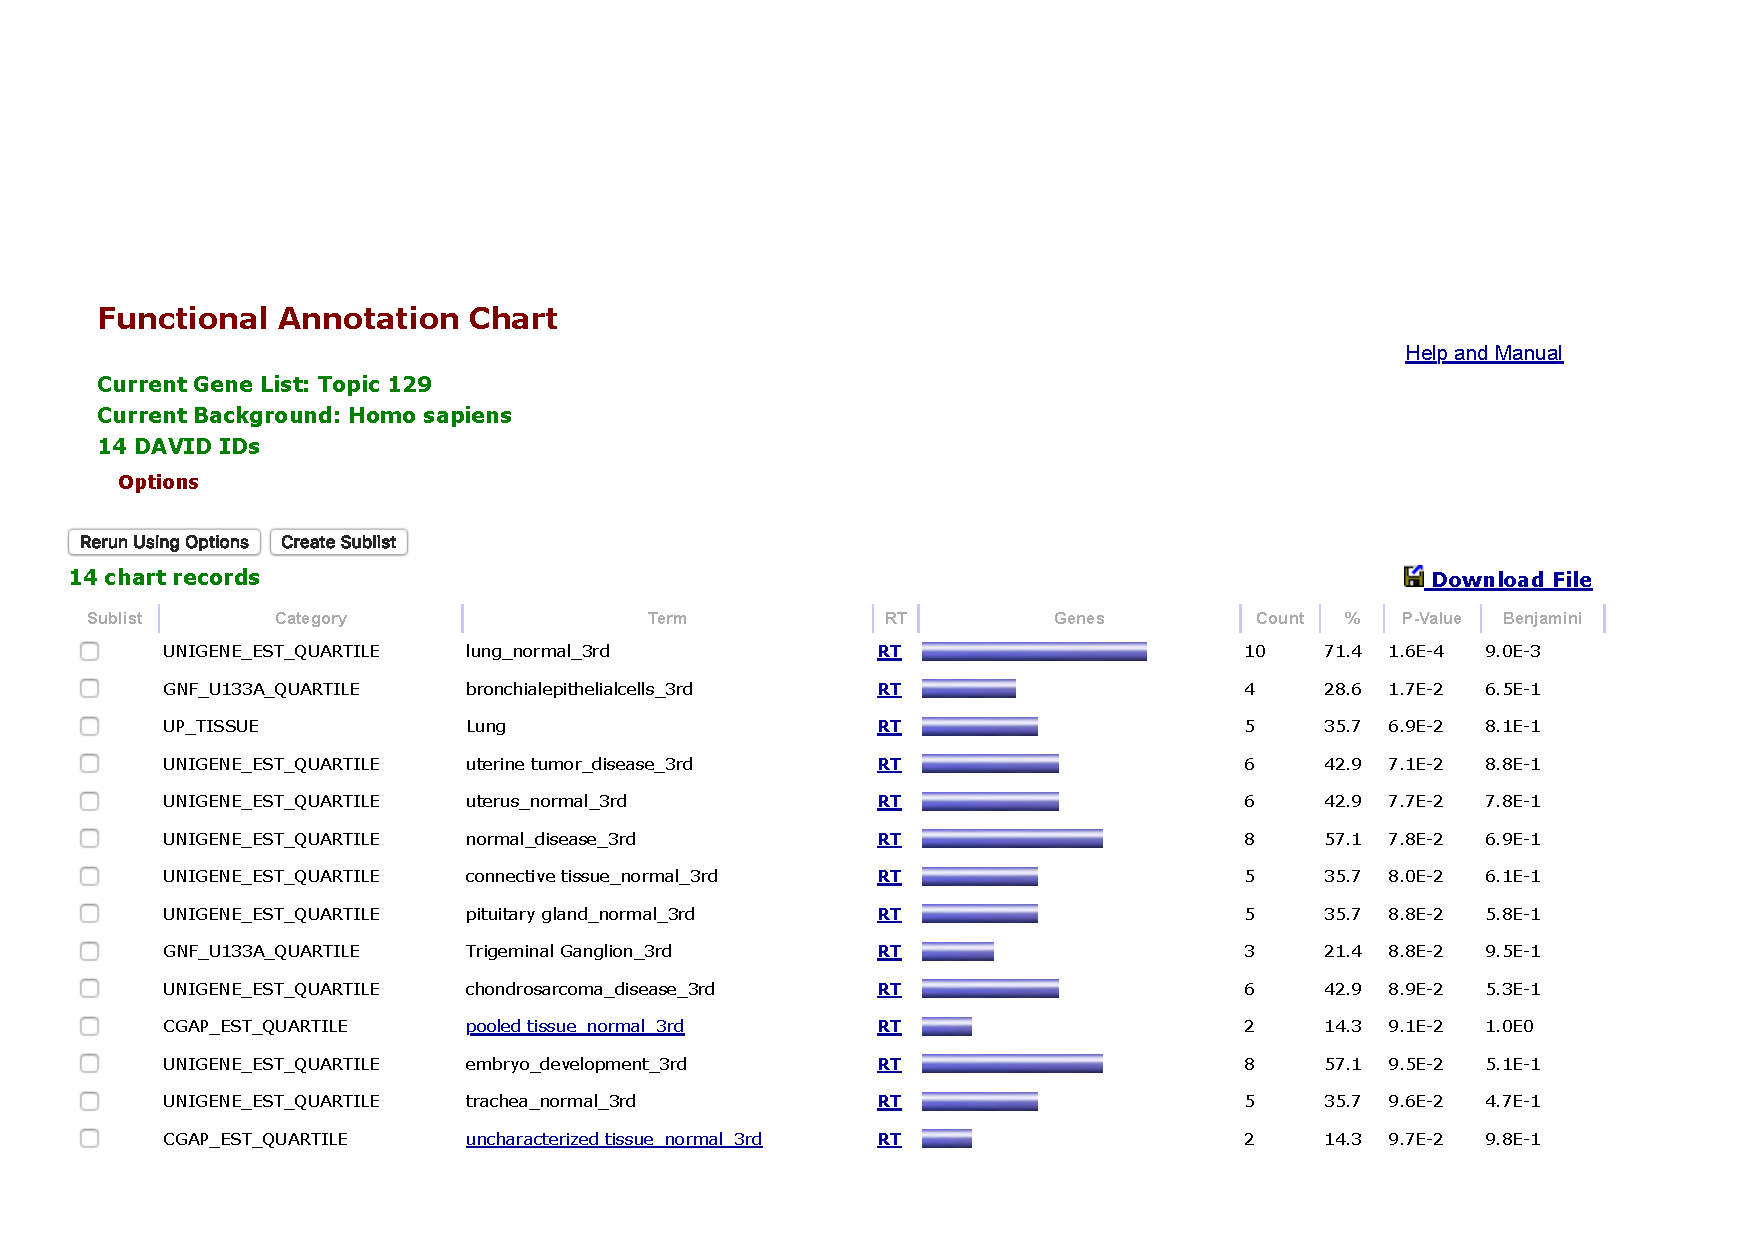
\includegraphics[width=0.8\linewidth]{pictures/topic/merged/DAVID_lung.pdf}
    \caption{Caption}
    \label{fig:topic/merged/DAVID_lung}
\end{figure}

\begin{figure}[htb!]
    \centering
    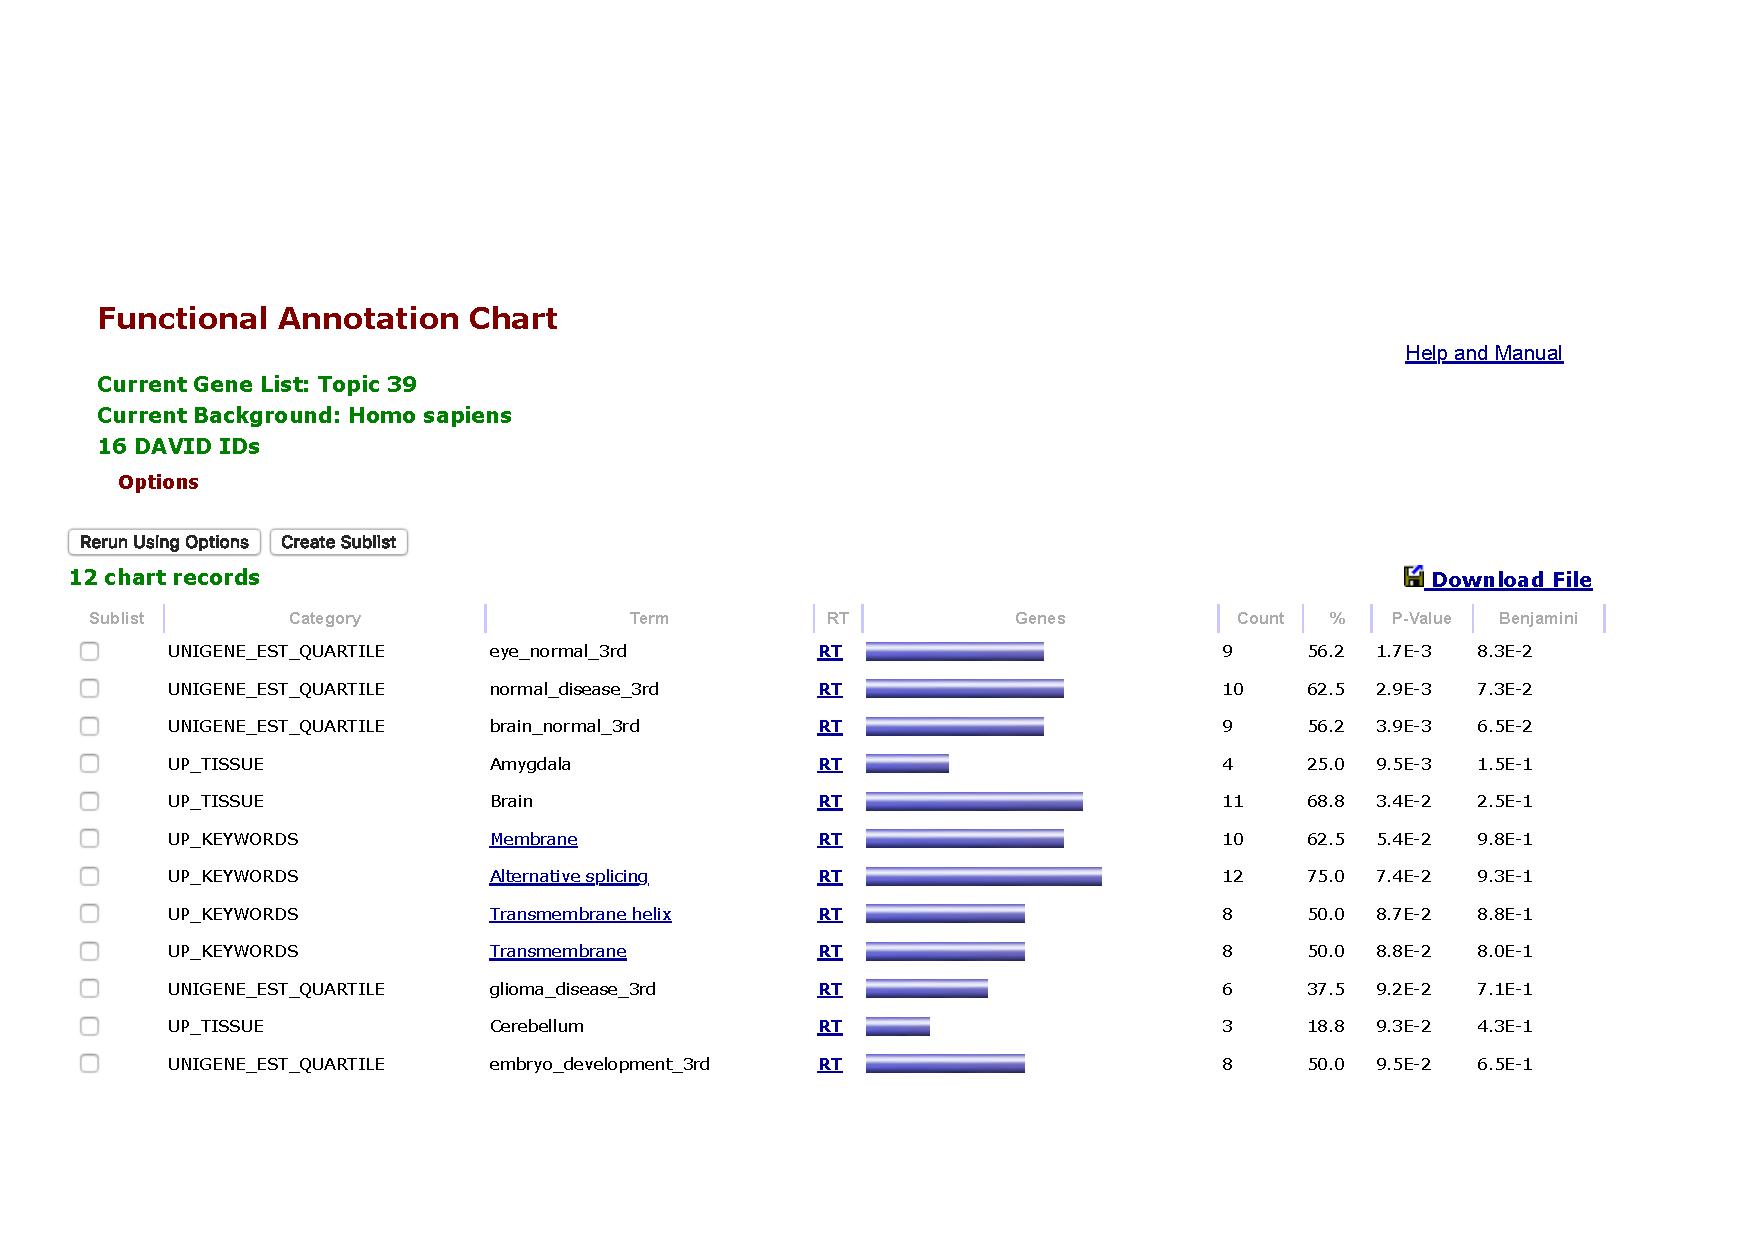
\includegraphics[width=0.8\linewidth]{pictures/topic/merged/DAVID_brain.pdf}
    \caption{Caption}
    \label{fig:topic/merged/DAVID_brain}
\end{figure}

\begin{figure}[htb!]
    \centering
    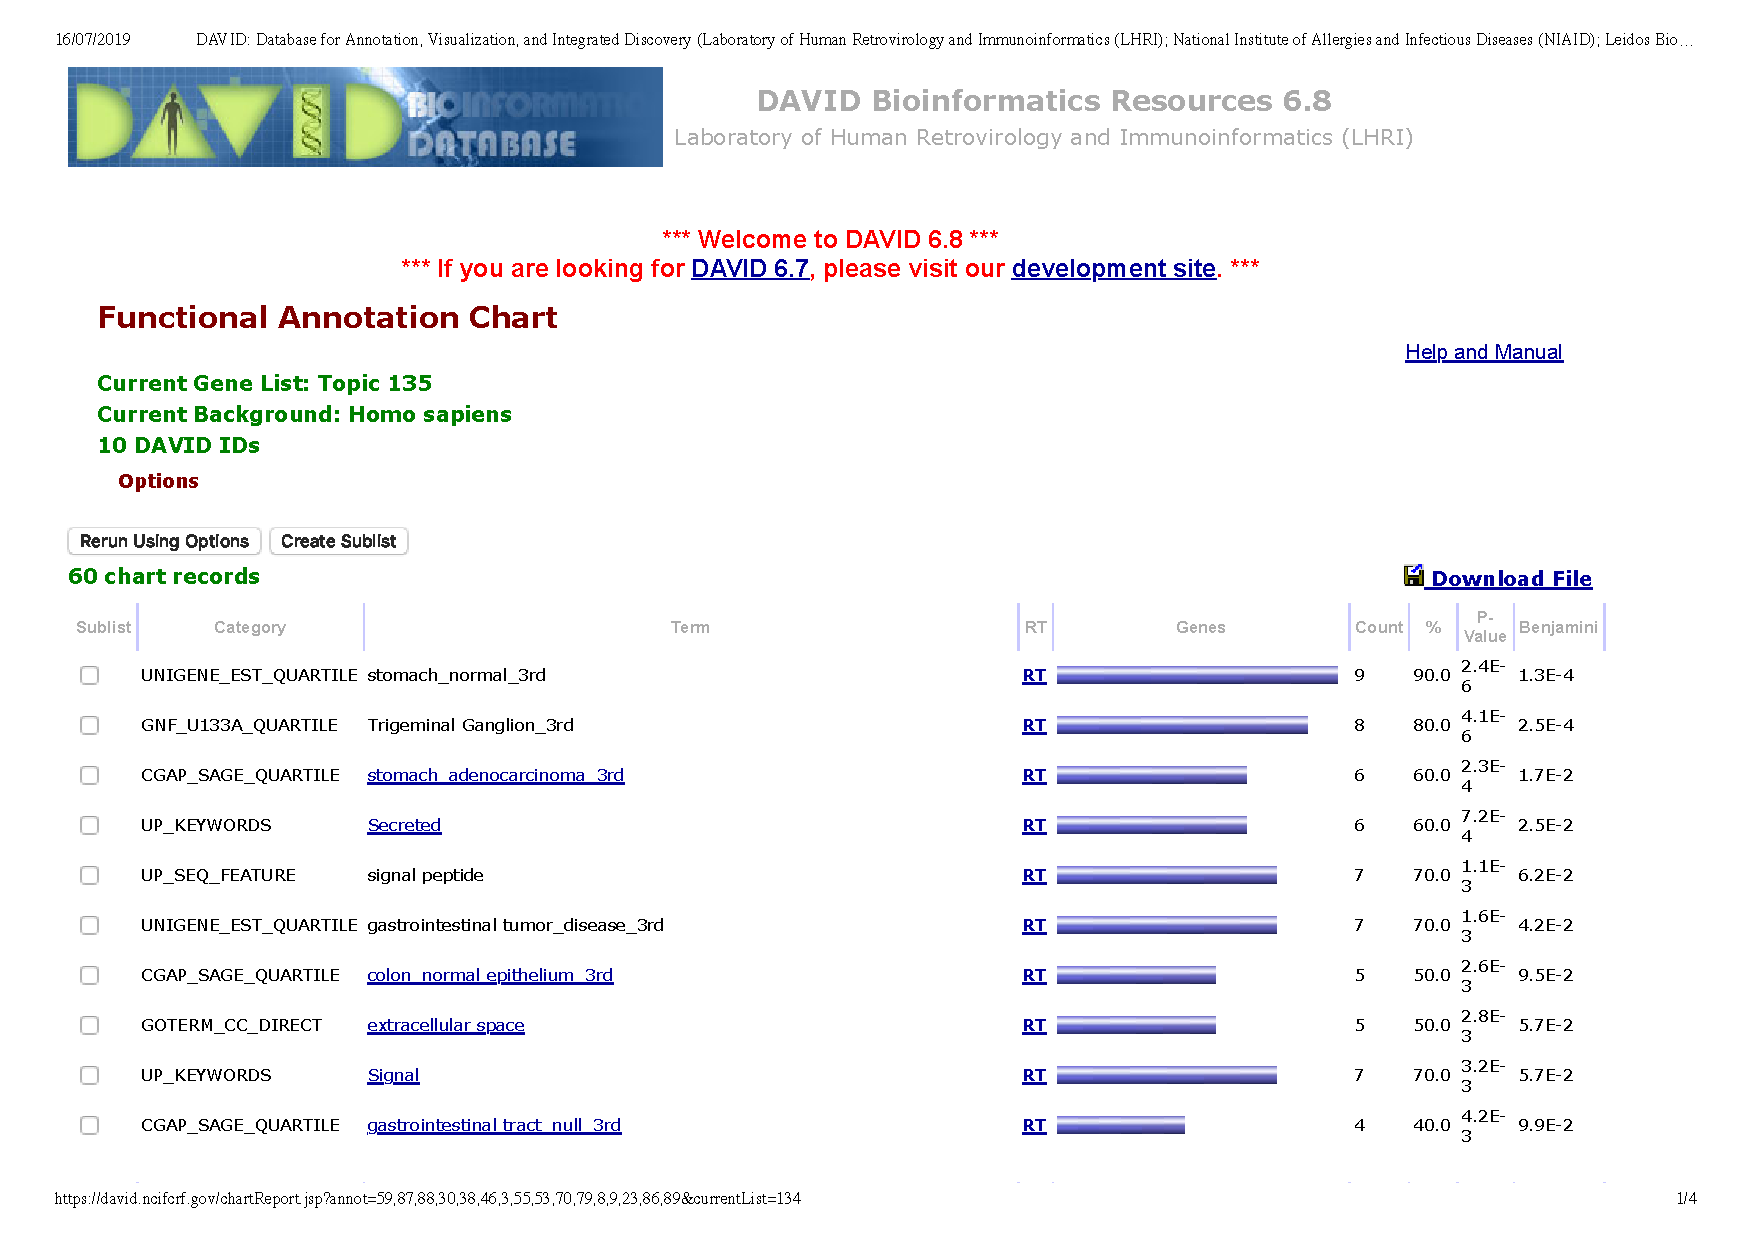
\includegraphics[width=0.8\linewidth]{pictures/topic/merged/DAVID_stomach.pdf}
    \caption{Caption}
    \label{fig:topic/merged/DAVID_stomach}
\end{figure}